% Totoro sitting in the snow
% By Noa Hoffmann and Pascal Günthner, 21.12.2020
\documentclass[tikz,11pt]{{standalone}}
\usepackage[T1]{fontenc}
\usepackage{helvet}
\usepackage{sans}
\usetikzlibrary{%
    positioning
%   shapes, shadows, patterns, calc,
%   decorations.shapes,
%   decorations.fractals,
%   decorations.markings,
%   decorations.pathmorphing
}
\tikzset{
    every node/.style = {
        rectangle, draw=black, thick,
        fill opacity = 0.5, text opacity = 1,
        font=\small, 
        outer sep=0pt,% <-- this eliminate your problem
    }
}

\begin{document}

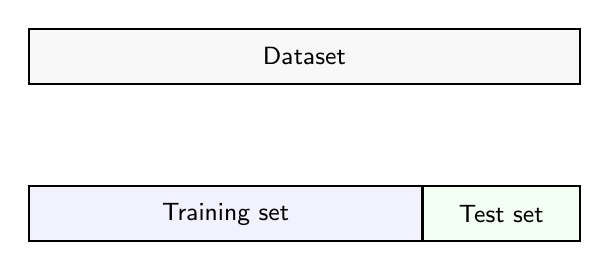
\begin{tikzpicture}
    \node[
        rectangle,
        draw,
        fill=gray!10,
        minimum width = 7cm,
        minimum height = 0.7cm
    ] (dataset) at (0, 0) {Dataset};
    \node[
        rectangle,
        draw,
        minimum width = 5cm,
        minimum height = 0.7cm,
        fill=blue!10,
        below=2cm of dataset.west,
        anchor=west
    ] (training) {Training set};
    \node[
        rectangle,
        draw,
        minimum width = 2cm,
        minimum height = 0.7cm,
        fill=green!10,
        right=0cm of training
    ] (test) {Test set};
    % \node[
    %     rectangle,
    %     draw,
    %     minimum width = 5cm,
    %     minimum height = 0.7cm,
    %     fill=blue!10,
    %     below=2cm of dataset.west,
    %     anchor=west
    % ] (training) {Training set};
    % \node[
    %     rectangle,
    %     draw,
    %     minimum width = 2cm, 
    %     minimum height = 0.7cm,
    %     fill=green!10,
    %     right=0cm of training
    % ] (test) {Test set};
\end{tikzpicture}

\end{document}
